\section{Slanted cell method}
\label{sec:slanted:method}

\begin{figure}
\centering
\begin{subfigure}{\textwidth}
	\centering
	\documentclass[tikz]{standalone}
\begin{document}
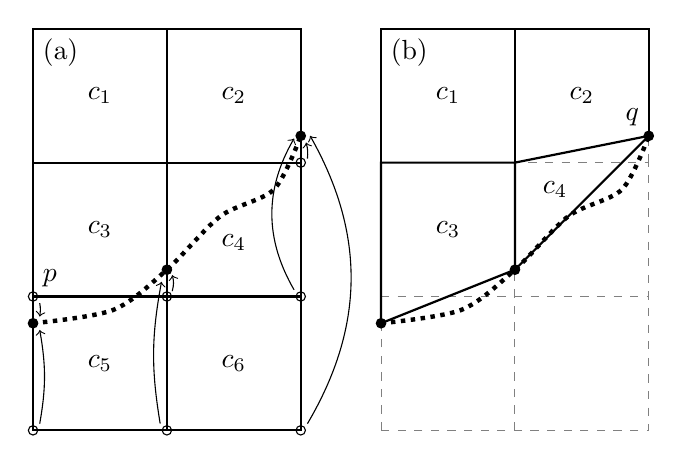
\begin{tikzpicture}[
  scale=0.17
]
\draw [thick] (0,0) rectangle (20, 20);
\draw [thick] (10,0) -- (10,20);
\draw [thick] (0,10) -- (20,10);
\draw [thick] (0,20) -- (0,30) -- (20,30) -- (20,20);
\draw [thick] (10,20) -- (10,30);
\draw [dotted, ultra thick] plot [smooth] coordinates {(0,8) (6, 9) (10,12) (14,16) (18,18) (20,22)};
\fill (0,8) circle [radius=0.4];
\fill (10,12) circle [radius=0.4];
\fill (20,22) circle [radius=0.4];
\draw (0,0) circle [radius=0.35];
\draw (0,10) circle [radius=0.35] node [anchor=south west] {$p$};
\draw (10,0) circle [radius=0.35];
\draw (10,10) circle [radius=0.35];
\draw (20,0) circle [radius=0.35];
\draw (20,10) circle [radius=0.35];
\draw (20,20) circle [radius=0.35];
\draw [->] (0.5,9.5) to [bend left=10] (0.5,8.5);
\draw [->] (0.5,0.5) to [bend right=10] (0.5,7.5);
\draw [->] (9.5,0.5) to [bend left=10] (9.6,11.1);
\draw [->] (10.4,10.4) to [bend right=15] (10.4,11.6);
\draw [->] (19.5,10.5) to [bend left=30] (19.5,21.8);
\draw [->] (20.5,0.5) to [bend right=30] (20.7,22);
\draw [->] (20.5,20.3) to [bend right=10] (20.4,21.5);
\node at (5,25) {$c_1$};
\node at (15,25) {$c_2$};
\node at (5,15) {$c_3$};
\node at (15,14) {$c_4$};
\node at (5,5) {$c_5$};
\node at (15,5) {$c_6$};

\node [below right] at (0,30) {(a)};

\draw [white] (20.6,0) rectangle (20.7,0);

\begin{scope}[shift={(26,0)}]
\draw [dashed, gray] (0,0) rectangle (20, 20);
\draw [dashed, gray] (10,0) -- (10,20);
\draw [dashed, gray] (0,10) -- (20,10);
\draw [dashed, gray] (20,20) -- (20,30);

\draw [thick] (0,8) -- (0,20) -- (10,20) -- (10,12) -- (0,8);
\draw [thick] (10,20) -- (20,22) -- (10,12);
\draw [thick] (0,20) -- (0,30) -- (20,30) -- (20,22);
\draw [thick] (10,20) -- (10,30);
\draw [dotted, ultra thick] plot [smooth] coordinates {(0,8) (6, 9) (10,12) (14,16) (18,18) (20,22)};
\fill (0,8) circle [radius=0.4];
\fill (10,12) circle [radius=0.4];
\fill (20,22) circle [radius=0.4] node [anchor=south east] {$q$};
\node at (5,25) {$c_1$};
\node at (15,25) {$c_2$};
\node at (5,15) {$c_3$};
\node at (13,18) {$c_4$};

\node [below right] at (0,30) {(b)};
\end{scope}
\end{tikzpicture}
\end{document}

	\phantomsubcaption\label{fig:slanted:construct-mesh:before}
	\phantomsubcaption\label{fig:slanted:construct-mesh:after}
\end{subfigure}
\caption{Illustration of a slanted cell mesh
(\subcaptionref{fig:slanted:construct-mesh:before}) before, and
(\subcaptionref{fig:slanted:construct-mesh:after}) after construction.
	The terrain surface, denoted by a heavy dotted line, intersects a uniform rectangular mesh comprising six cells, $c_1, \ldots, c_6$.
	The cell vertices, marked by open circles, are moved to the points at which the terrain intersects vertical cell edges, marked by filled circles.  Cells that have no volume are removed.  Where a cell has two vertices occupying the same point, the zero-length edge that joins those vertices is removed.
	In this illustration, cells $c_5$ and $c_6$ are removed because they have no volume, and the zero-length edge at point $q$ is removed to create a triangular cell, $c_4$.
	Point $p$ is moved down because it is within $2 \Delta z/5$ of the surface, avoiding the creation of a thin cell.}
\label{fig:slanted:construct-mesh}
\end{figure}

The slanted cell method is straightforward, and slanted cell meshes are always free of mesh tangling by construction.
Starting from a uniform rectangular mesh, all cell vertices that lie beneath the orography are moved up to the surface.
Additionally, to avoid creating very thin cells, all vertices up to $2 \Delta z/5$ above the orography can be moved down to the surface.
Where all four of a cell's vertices are moved, the cell has zero volume and so it is removed.  Where two vertices at the same horizontal location are moved up to the surface they will occupy the same point; this results in a zero-length edge that is removed to create a triangular cell.
Figure~\ref{fig:slanted:construct-mesh} shows how a $2 \times 3$-cell, uniform rectangular mesh is transformed into a slanted cell mesh.  Cells $c_5$ and $c_6$ are removed because they have zero volume, and the zero-length edge at point $q$ is removed to create a triangular cell, $c_4$.
Point $p$ is moved down because it is within $2\Delta z/5$ of the surface, avoiding the creation of a very thin cell.
We have not explored the sensitivity of results using values other than $2\Delta z/5$, but we did find that this approach reduces numerical errors on some meshes with very thin slanted cells.

The slanted cell method does generate some small cells but, unlike the cut cell method, the width of slanted cells is never altered.
Since a no normal flow condition is imposed at the lower boundary, flow must be parallel to the surface and there is only very weak flow across the long, upper face of slanted cells.
Hence, slanted cell meshes should not suffer from severe time-step constraints associated with arbitrarily small cut cells because slanted cells are never shortened in the direction of flow.
An example of a slanted cell mesh is illustrated in figure~\ref{fig:slanted:resting:meshes:slantedCell} for comparison with the equivalent BTF (figure~\ref{fig:slanted:resting:meshes:btf}), SLEVE (figure~\ref{fig:slanted:resting:meshes:sleve}), and cut cell (figure~\ref{fig:slanted:resting:meshes:cutCell}) meshes, with the same mesh spacing and mountain profile used for all meshes.
